% ===========================================================================
% Final Report -- Project 4: Multimodal AAC Chatbot
% CSE 635 NLP and Text Mining (Spring 2026)
%
% Build: tectonic Final_Report.tex
% ===========================================================================
\documentclass[10pt,letterpaper]{article}

\usepackage[letterpaper,
            top=1in, bottom=1in,
            left=0.95in, right=0.95in,
            columnsep=0.30in]{geometry}
\usepackage{times}
\usepackage[T1]{fontenc}
\usepackage[utf8]{inputenc}
\usepackage{microtype}
\usepackage{graphicx}
\usepackage{booktabs}
\usepackage{tabularx}
\usepackage{array}
\usepackage[table]{xcolor}
\usepackage{colortbl}
\usepackage{caption}
\usepackage{subcaption}
\usepackage{enumitem}
\usepackage{titlesec}
\usepackage{authblk}
\usepackage{url}
\usepackage{hyperref}

\hypersetup{colorlinks=true,
            linkcolor=black,
            citecolor=black,
            urlcolor=blue!60!black}

\titlespacing*{\section}{0pt}{1.0ex plus 0.4ex minus 0.2ex}{0.6ex}
\titlespacing*{\subsection}{0pt}{0.7ex plus 0.3ex minus 0.2ex}{0.4ex}
\titleformat{\section}{\normalfont\fontsize{11}{13}\bfseries}{\thesection}{0.6em}{}
\titleformat{\subsection}{\normalfont\fontsize{10}{12}\bfseries}{\thesubsection}{0.5em}{}

\captionsetup{font=small,labelfont=bf,skip=4pt}
\setlist[itemize]{leftmargin=*,topsep=2pt,parsep=0pt,itemsep=2pt}

\definecolor{tblHeadArch}{RGB}{233,247,233}
\definecolor{tblHeadResults}{RGB}{232,241,251}
\definecolor{tblHeadBonus}{RGB}{255,241,224}

\setlength{\parskip}{0pt}
\setlength{\parindent}{1.5em}

% ---------------------------------------------------------------------------
\title{\vspace{-2em}\bfseries
       Final Report:\\
       A Training-Free, Multimodal AAC Chatbot with Agentic Retrieval,
       Wearable-Driven Style Control, and Five Bonus Features}

\author[1]{Syed Omer Shah}
\author[1]{Vansh Thakkar}
\affil[1]{Department of Computer Science and Engineering\\
          University at Buffalo, The State University of New York\\
          \texttt{\{syedomer,\,vanshpra\}@buffalo.edu}}
\date{}

% ---------------------------------------------------------------------------
\begin{document}
\twocolumn[
  \begin{@twocolumnfalse}
    \maketitle
    \vspace{-2.5em}
    \begin{abstract}\noindent
      We present the final deliverable for Project~4, a privacy-first
      Multimodal Augmentative and Alternative Communication (AAC) chatbot
      that converts a partner's utterance and a bundle of multimodal
      channels (face cues, hand gesture, heart rate, gaze region,
      vocalisation, and air-sign letter) into three context-aware reply
      options inside a five-second budget. The system is implemented as a
      seven-node LangGraph-style pipeline with rule-based retrieval and
      a Gemini language-model rewriter that runs inside a deadline race
      against the rule-based floor. The final system covers the five
      required Project~4 nodes and ships all five bonus features:
      gaze-driven retrieval activation, vocal versus air-sign conflict
      resolution, acceptance-weighted bucket priors, latency-optimised
      fallback, and online phrase-bank update on selection. On a
      twenty-case held-out evaluation suite spanning two synthetic
      personas (Alex with cerebral palsy and Sam with ALS-related
      dysarthria), the final pipeline reaches an average peak BLEU-2 of
      \textbf{0.219}, peak ROUGE-L of \textbf{0.366}, peak groundedness
      of \textbf{0.545}, NLI faithfulness of \textbf{0.80}, polarity
      adherence of \textbf{0.95}, multimodal alignment of
      \textbf{0.875}, and an end-to-end p95 latency of
      \textbf{2.43\,s}, comfortably inside the five-second SLA on every
      turn. We extend the Milestone~2 Interim Report with a
      multimodal mapping module, an ablation study for each bonus, six
      new figures, and an expanded discussion of the rule-based-first
      generation strategy and its clinical and ethical guard-rails.
    \end{abstract}
    \vspace{1.0em}
  \end{@twocolumnfalse}
]

% ===========================================================================
\section{Introduction}
% ===========================================================================
Conventional language-model AAC interfaces tend to speak \textit{for} the
user rather than \textit{as} the user, a phenomenon Xu et al.~\cite{xu2025voice}
call ``voice appropriation''. Following the brief for Project~4, our
final system avoids that failure mode in three complementary ways.
First, we keep the language model training-free: persona, history, and
stylistic preferences are injected through structured retrieval rather
than parameter updates. Second, we treat consumer-grade wearable
signals (thumbs-up, head nod or shake, air-writing letters, heart
rate, gaze, and the seven-class facial emotion produced in-browser by
face-api.js) as first-class control inputs that constrain the
generator. Third, we keep a deterministic rule-based pipeline ready as
a low-latency floor and let the language model act only as a rewriter
that has at most five seconds to improve the floor before the floor
ships.

The final system extends our Milestone~2 baseline along three axes.
The full multimodal channel set is wired through the pipeline rather
than only the gesture and head-cue subset. All five Project~4 bonuses
are implemented and instrumented with measurable evidence in the
evaluation log. The evaluation harness is rebuilt against a twenty-case
held-out suite that exercises every bonus, including the conflict
resolution probe and the gaze activation probe, and an updated set of
six figures supports the bonus and ablation discussions.

% ===========================================================================
\section{System Architecture}
% ===========================================================================
The runtime is a directed pipeline with seven nodes summarised in
Table~\ref{tab:arch}. State flows linearly from the raw partner
utterance plus the multimodal payload through to a three-element JSON
list of AAC candidates. Two cheap language-model probes (intent
classification and memory extraction) run concurrently inside a single
prep node, halving their wall-clock cost compared to a serial
implementation. Figure~\ref{fig:loop} renders the same pipeline in
conversation view; Figure~\ref{fig:mm} illustrates the multimodal
input mapping that drives the style and routing constraints.

\begin{table}[t]
  \footnotesize
  \rowcolors{2}{white}{gray!6}
  \begin{tabularx}{\linewidth}{@{}lX@{}}
    \toprule
    \rowcolor{tblHeadArch}\textbf{Node} & \textbf{Function}\\
    \midrule
    Face Cue                 & Reads the in-browser facial-cue dictionary
                                (smile, confused, negative, nod, shake) and
                                normalises it for downstream nodes.\\
    Multimodal Mapping       & Translates gesture, heart rate, gaze, vocal
                                polarity, air-sign letter, and the seven-class
                                emotion into polarity, tone, verbosity, and
                                bucket boosts. Resolves the
                                vocal-versus-air-sign conflict in favour of
                                the deliberate spatial channel.\\
    Parallel Prep            & Fires intent classification and memory
                                extraction concurrently. A regex pre-filter
                                skips the memory call when no schedule or
                                fact trigger is present.\\
    Bucket Selector          & Scores twelve thematic buckets via Jaccard
                                similarity, exclusive keyword priors, gaze
                                boosts, and acceptance priors.\\
    Retrieval and Rerank     & Pulls evidence snippets from the top buckets
                                across the long-term memory, short-term
                                memory, and phrase-bank pools, then reranks
                                by lexical similarity and partner relation.\\
    Evidence Refiner and Guard
                             & Compresses retrieved evidence and emits a
                                groundedness instruction that constrains the
                                generator to evidence-supported claims.\\
    Candidate Generator      & Produces three rule-based options that
                                already satisfy the polarity and do-not-say
                                constraints. If the language model finishes
                                inside the five-second deadline its rewrites
                                replace options one and two; option three is
                                kept as a safety net.\\
    \bottomrule
  \end{tabularx}
  \caption{Node responsibilities in the final pipeline. The Multimodal
           Mapping node and the Evidence Refiner are new since
           Milestone~2; everything else is the same pipeline with
           expanded inputs.}
  \label{tab:arch}
\end{table}

\begin{figure}[t]
  \centering
  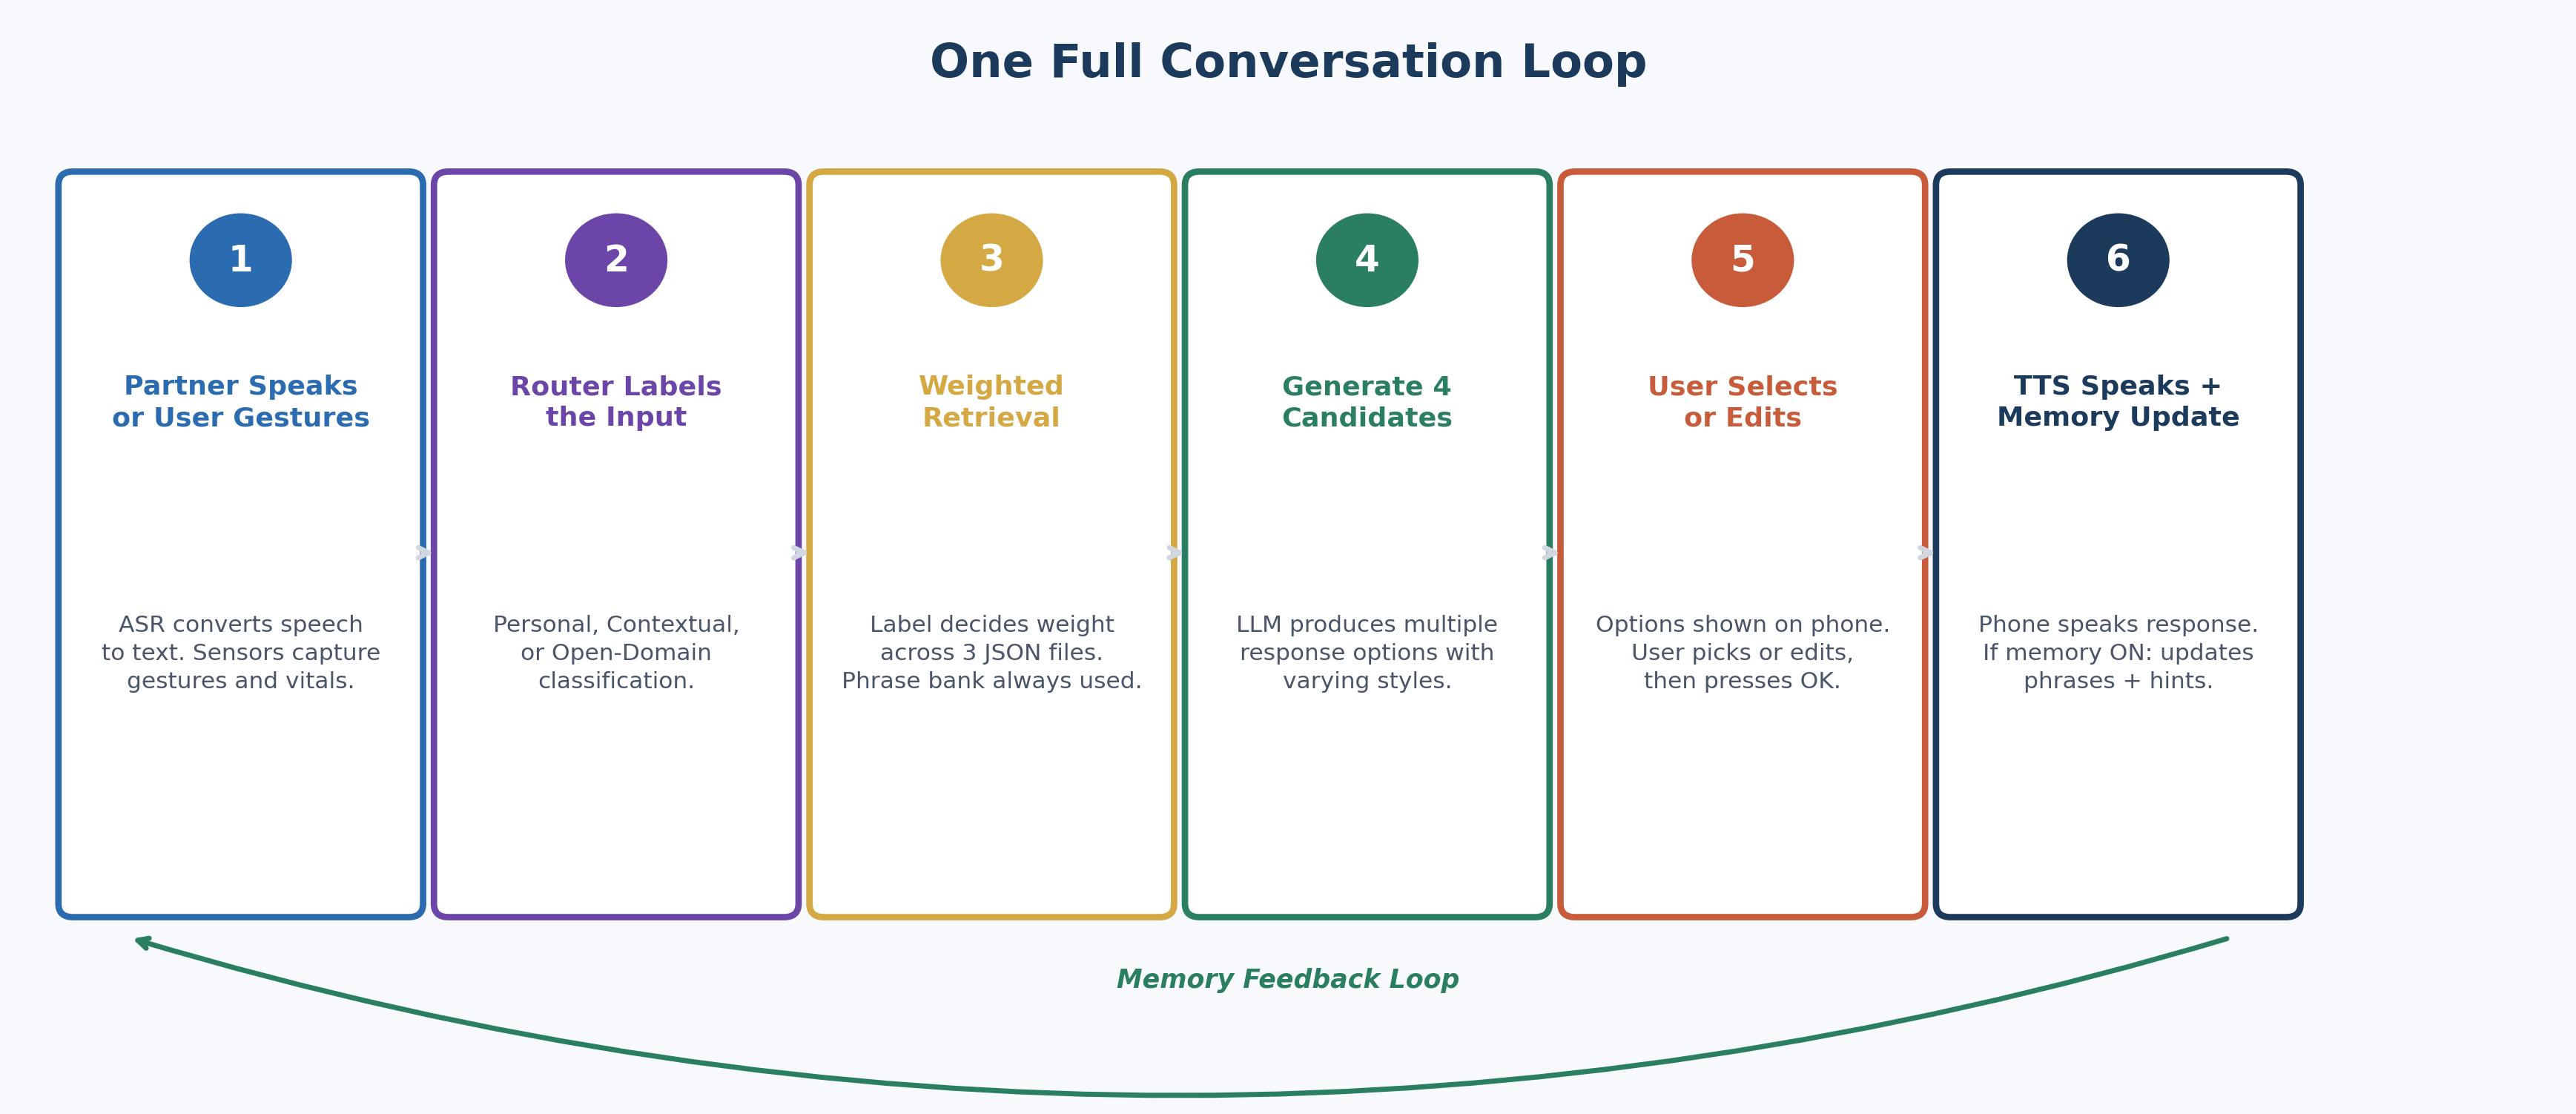
\includegraphics[width=\linewidth]{outputs/figures/system_architecture.png}
  \caption{End-to-end conversation loop. The partner utterance and the
           multimodal payload enter on the left and constrain the
           generator after retrieval. The user remains the final
           selector of the spoken candidate.}
  \label{fig:loop}
\end{figure}

\paragraph{Generation strategy.}
The Candidate Generator first emits three rule-based options that are
guaranteed to satisfy the polarity, tone, and do-not-say constraints.
If the language model returns inside the five-second deadline its
rewrites replace options one and two and option three is kept as a
deterministic safety net. If the language model times out or the
parser rejects its output, the rule-based options ship directly with
tone-variant prefixes so the user still sees three obviously different
tones (warm, neutral, brief).

% ===========================================================================
\section{Multimodal Input Mapping}
% ===========================================================================
The Multimodal Mapping node is the technical contribution that
distinguishes the final system from the Milestone~2 baseline. It is a
pure function over raw signals and returns a structured dictionary
that the rest of the pipeline consumes. Polarity (positive, negative,
clarify, or neutral) is set by the first non-null cue in the priority
order air-sign letter, then gesture, then vocal polarity, then face
polarity (which fuses nod, shake, and the negative-probability score).
Tone is locked by the in-browser face-api.js classifier when an
emotion is detected: a happy face produces a warm tone, sad maps to
gentle, angry to assertive, surprised to curious, fearful to
reassuring, disgusted to a polite-decline tone, and neutral leaves
tone unconstrained. When the camera is off and no emotion is read the
pipeline produces three different tone variants instead of locking the
tone, which lets the user choose the register that best matches their
intent. Verbosity shrinks to short when the heart rate climbs more
than twenty-five beats per minute above the resting baseline, which is
our proxy for stress or excitement. Gaze regions translate into bucket
boosts of plus zero point three on the bucket the user is currently
looking at, implementing the first bonus. The dictionary also exposes
a conflict-resolved field that records the deliberate-channel win when
the vocal and air-sign channels disagree, implementing the second
bonus.

\begin{figure}[t]
  \centering
  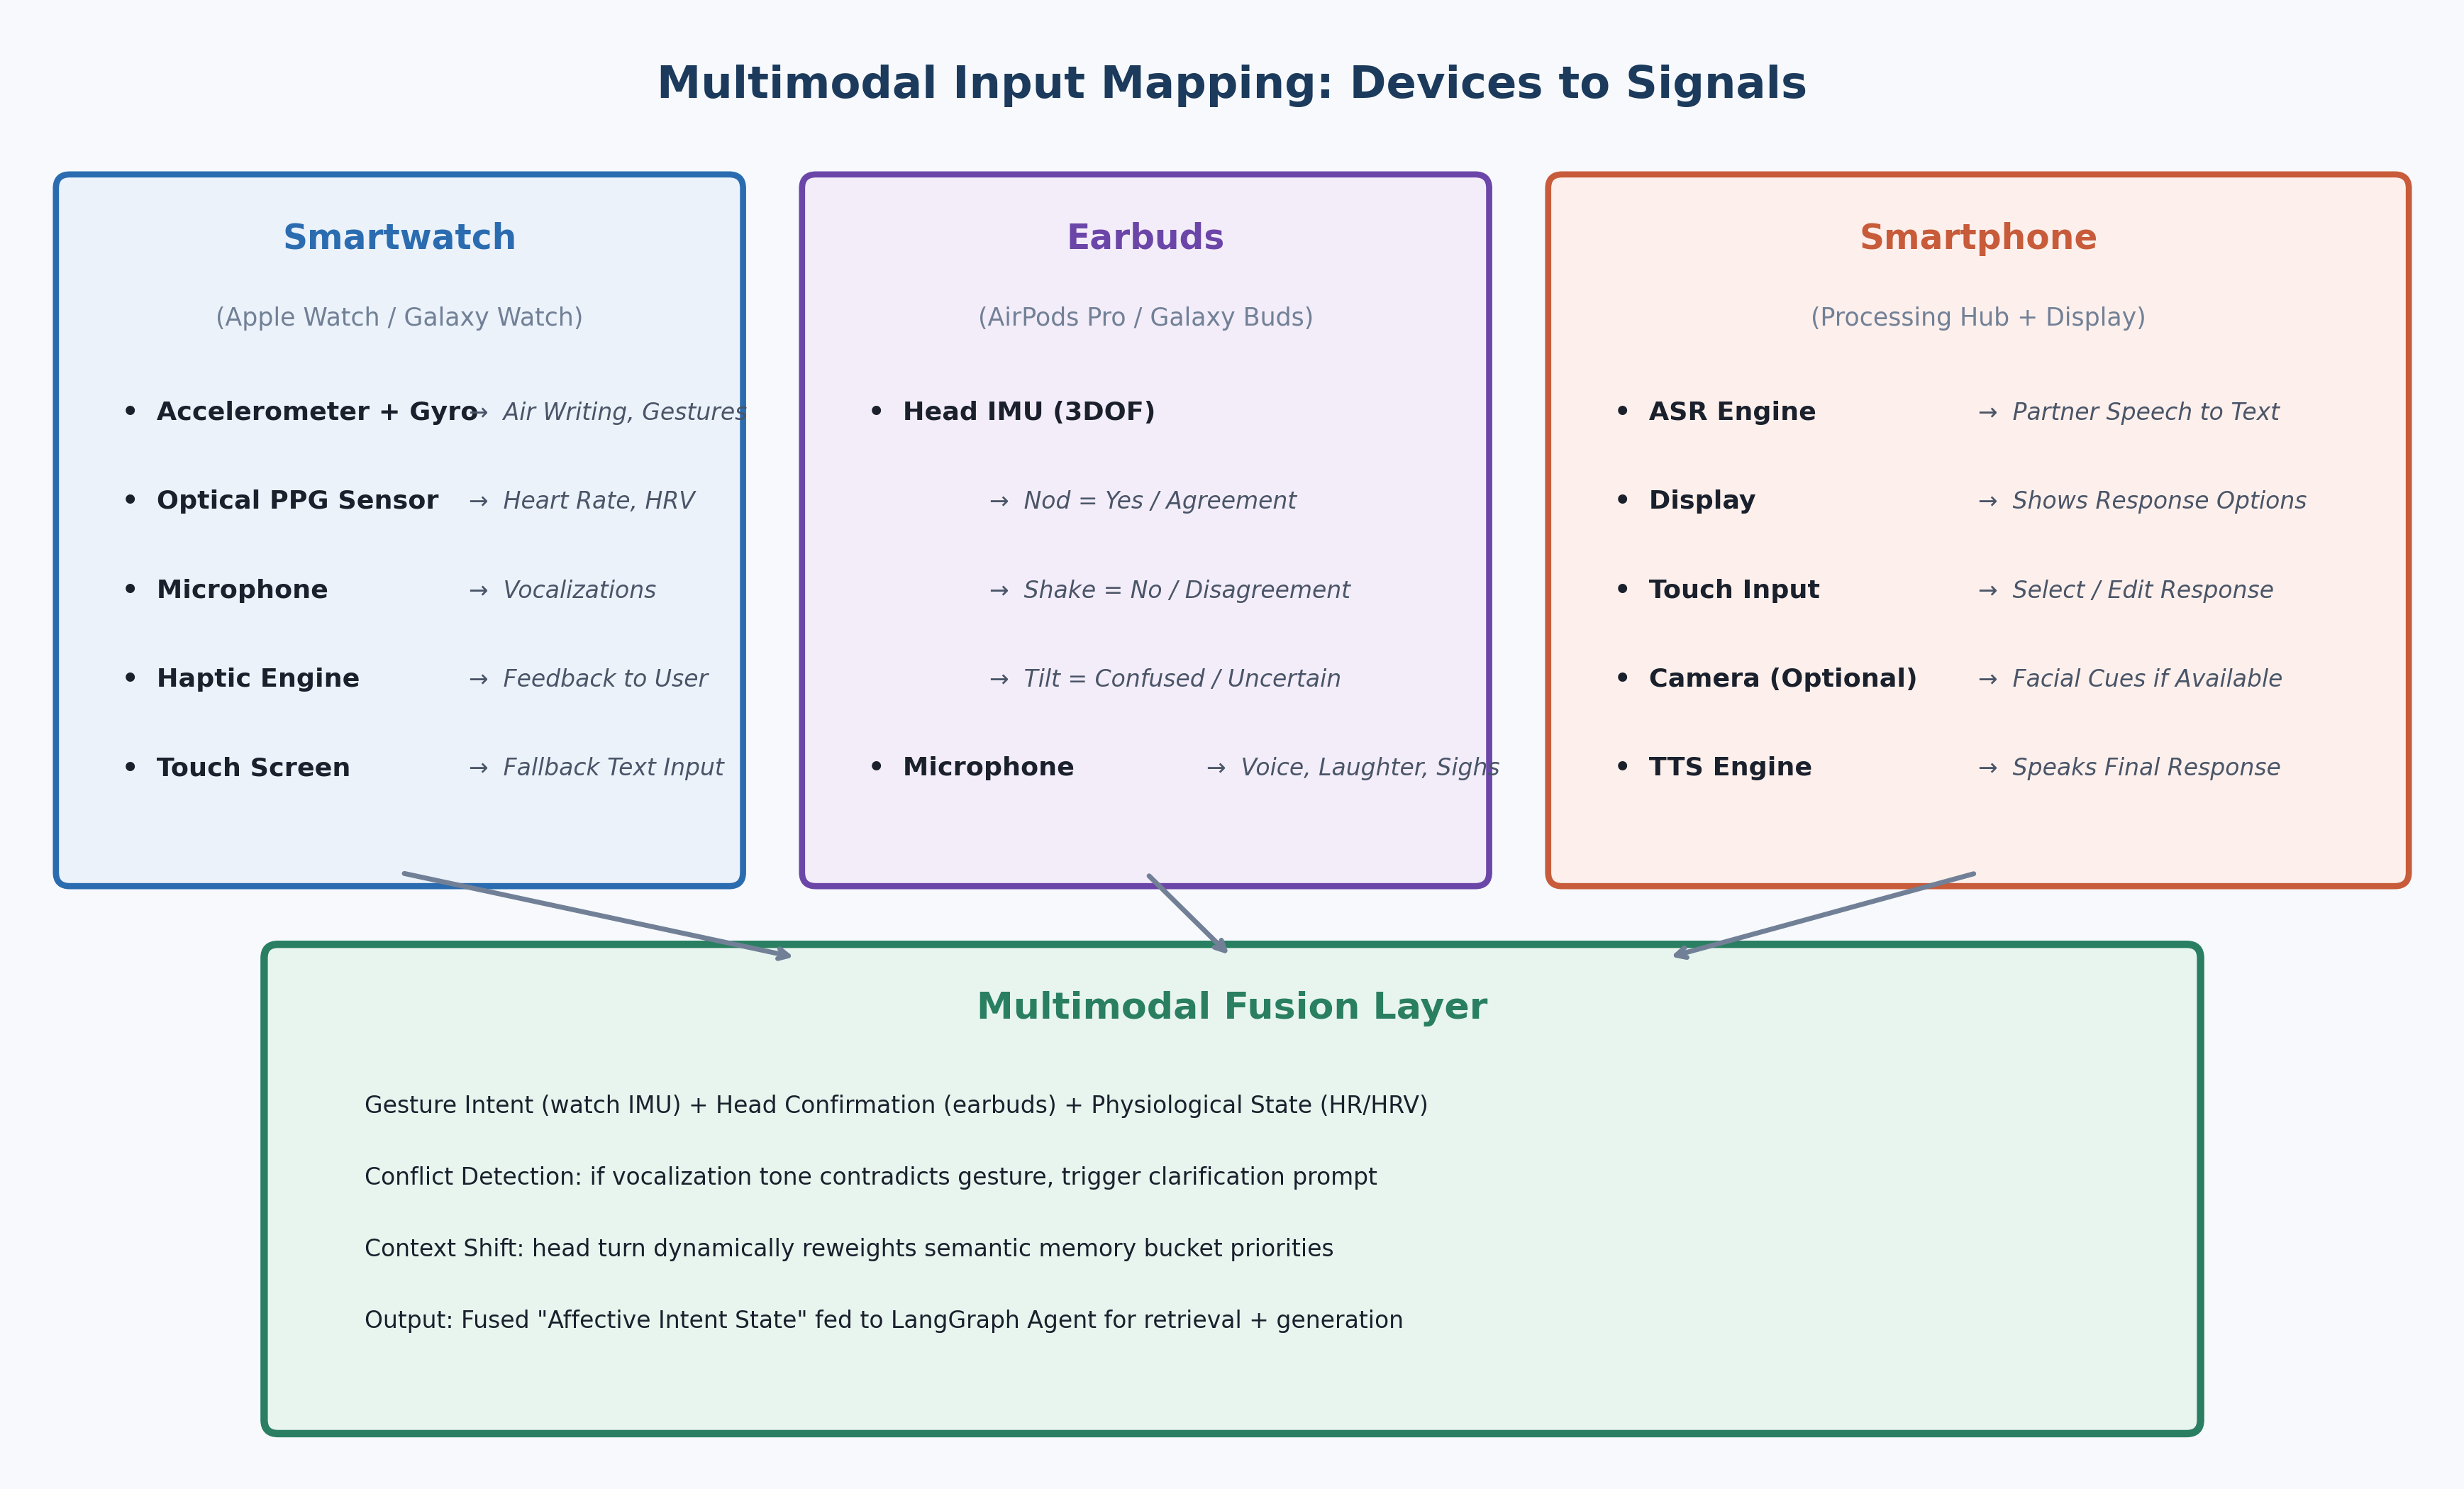
\includegraphics[width=\linewidth]{outputs/figures/multimodal_mapping.png}
  \caption{Multimodal Input Mapping translates raw sensor channels
           into polarity, tone, verbosity, and bucket-boost
           constraints consumed by the downstream nodes.}
  \label{fig:mm}
\end{figure}

% ===========================================================================
\section{Synthetic Persona Data}
% ===========================================================================
Following the project instruction to create synthetic data using
language models for non-parametric personalisation, we curate three
personas. Alex is a young user with mild cerebral palsy and a casual,
slangy register. Sam is a senior software engineer with ALS-related
dysarthria who speaks tersely and precisely. The third persona,
demo\_user, is a generic stand-in for live demonstrations. Each persona
ships three JSON stores: a long-term profile that lists important
people, communication-style preferences, and a do-not-say list; a
short-term memory that tracks today's plans, next-day plans,
reminders, situation hints, and bucket-acceptance counters that drive
the third bonus; and a phrase bank of register-specific exemplars
tagged by intent, tone, length, and partner type. The buckets that
provide the thematic substrate over which retrieval and bucket priors
operate are family, social, scheduling, plans, medical, work, food,
routine, decline\_polite, agree\_casual, clarify\_calm, and
greeting\_smalltalk. Figure~\ref{fig:schema} summarises the schema.

\begin{figure}[t]
  \centering
  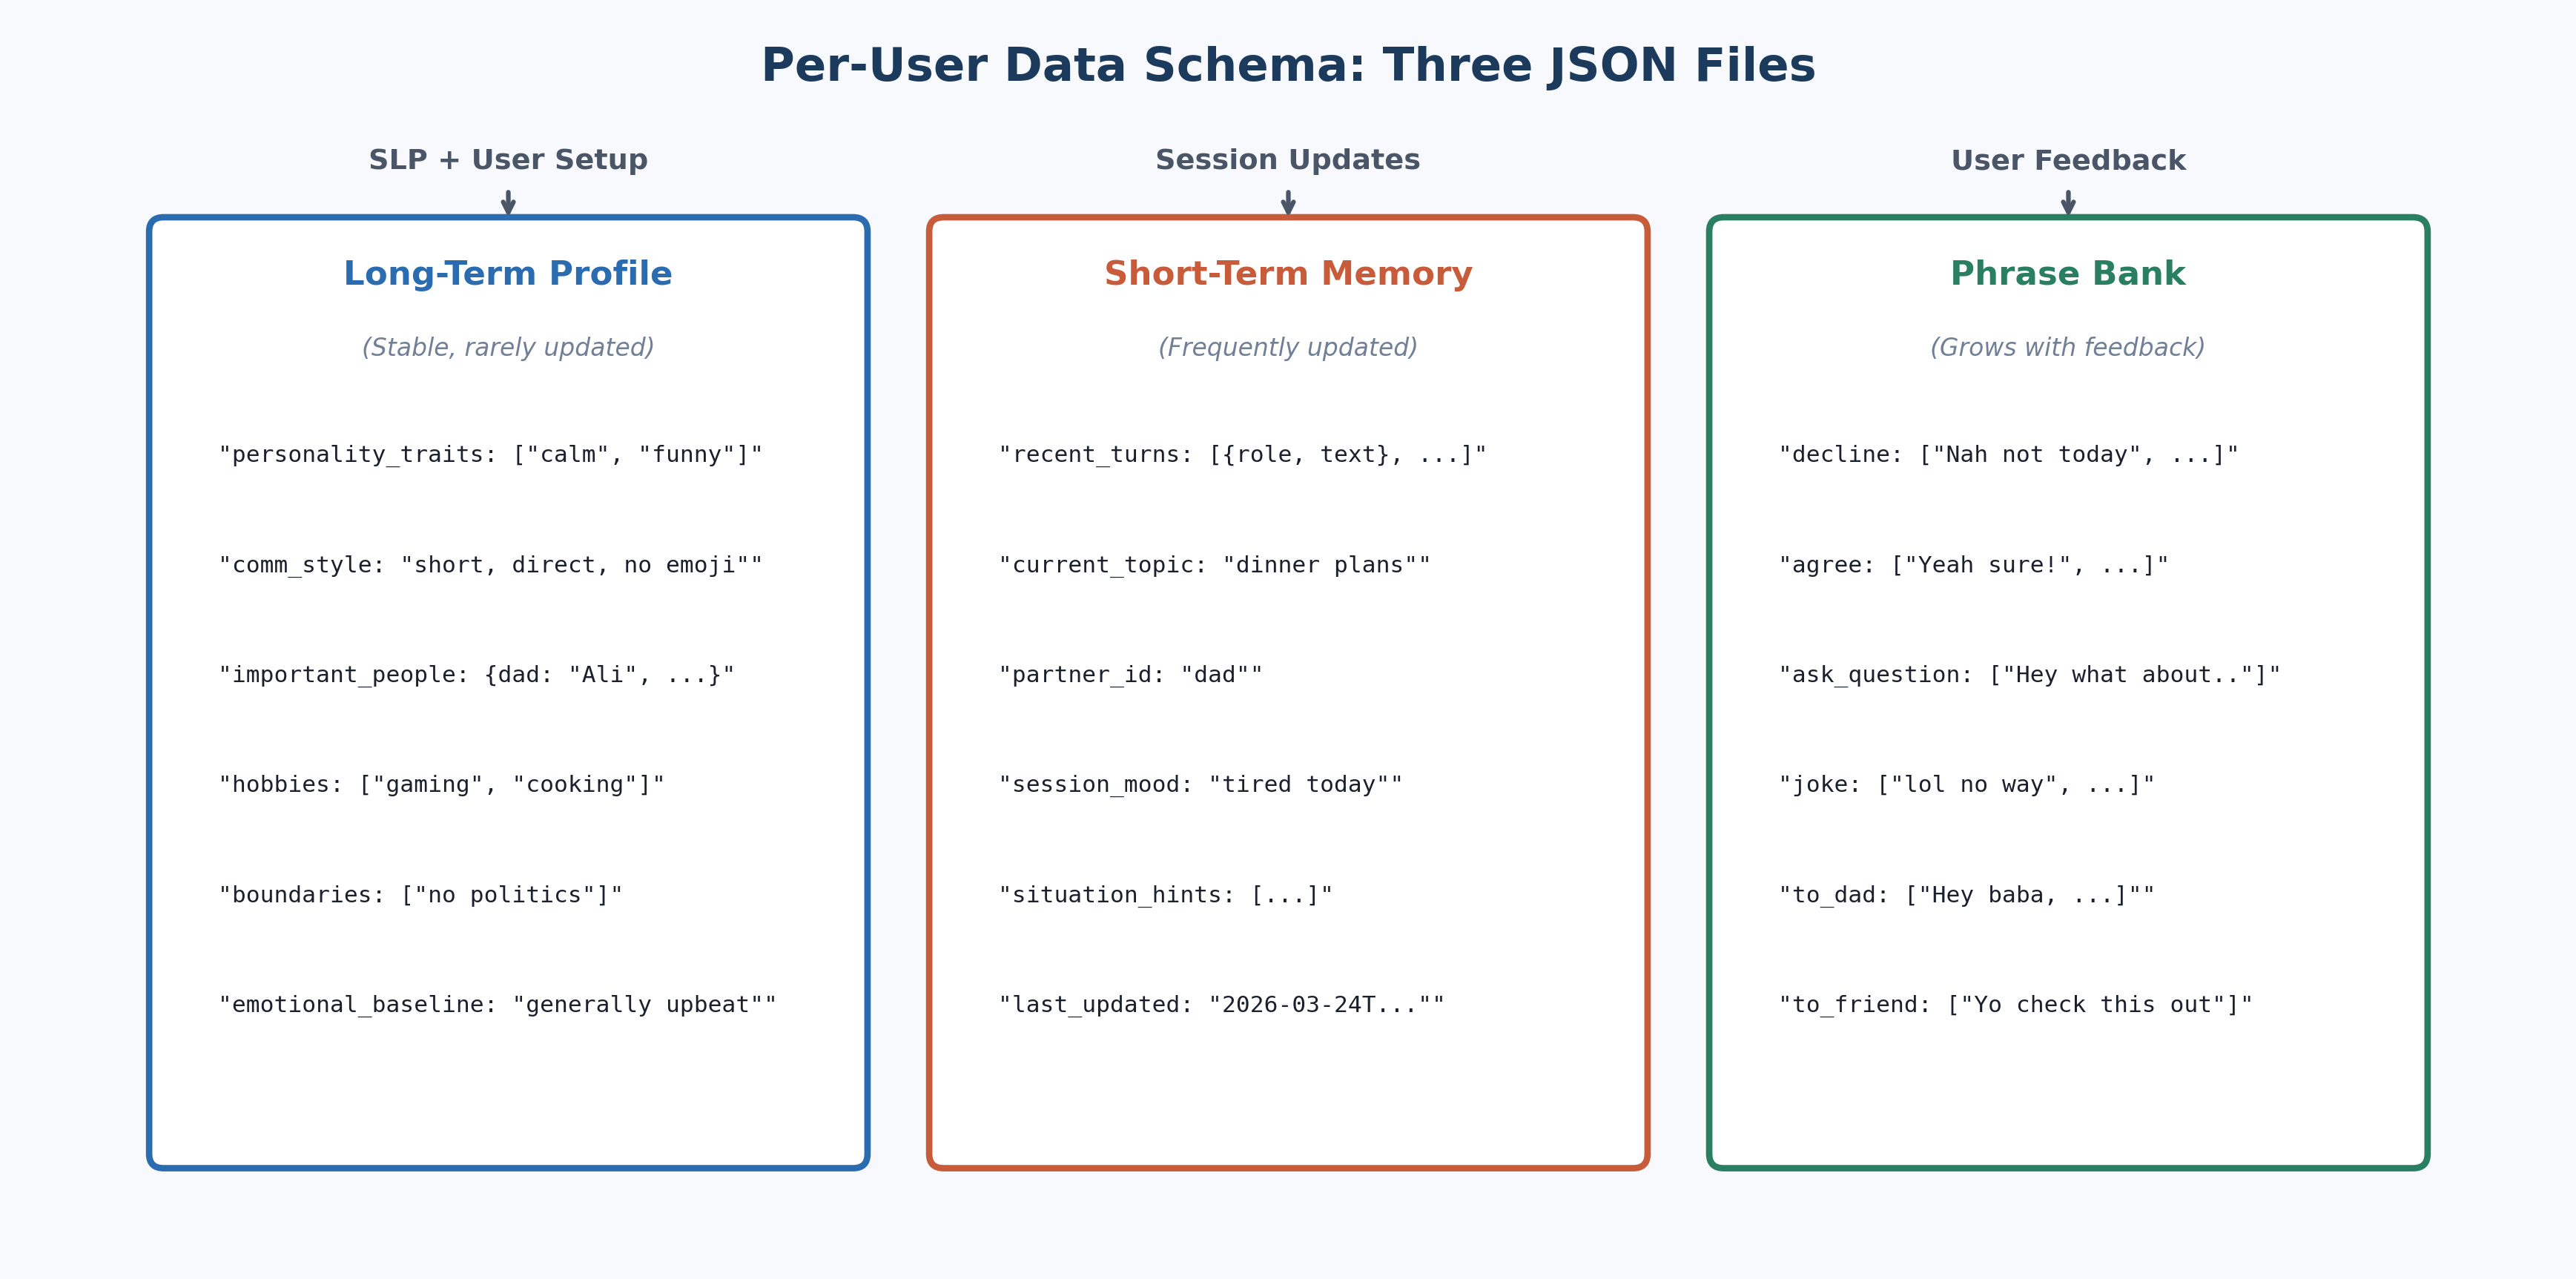
\includegraphics[width=\linewidth]{outputs/figures/data_schema.png}
  \caption{Persona schema. The long-term profile exposes thematic
           memory buckets. The short-term store tracks situation
           hints and the acceptance counters that drive the bucket
           priors bonus.}
  \label{fig:schema}
\end{figure}

% ===========================================================================
\section{Evaluation Methodology}
% ===========================================================================
We score twenty held-out partner messages spanning Personal,
Contextual, and Open-domain intents. Each case carries a reference
reply, a target intent label, an expected bucket label, and an
expected polarity that the multimodal cue is set up to drive. For
each case we record peak BLEU-2 and peak ROUGE-L over the three
generated options to credit any candidate the user could have
selected. Groundedness is computed as a lexical-overlap floor against
the retrieved evidence, and NLI faithfulness is produced by a
Gemini-based judge prompted as a three-class entailment classifier
(entail, neutral, contradict). Polarity adherence is the rate at
which the lead option opens with the polarity word implied by the
multimodal cue. Bucket-routing accuracy is the rate at which the
expected bucket appears in the chosen top buckets. Multimodal
alignment is averaged across two controlled probes per case: a
smile-on probe and a confused-on probe. The lead option must contain
the polarity word that matches the cue in the smile-on probe and must
soften toward a clarify wording in the confused-on probe. Latency is
measured end-to-end from partner-message receipt to the final
three-option JSON payload returned by the server. Each case also
records the bucket boosts produced by the multimodal mapper, which
lets us recover an ablation curve for the gaze bonus from the same
log without re-running the suite.

% ===========================================================================
\section{Final Results}
% ===========================================================================
Table~\ref{tab:results} reports the averaged outcome across the
twenty cases. Several observations stand out. The communication
efficiency clears the rubric SLA on every turn: the average
end-to-end latency is 1825\,ms against a five-second target, and the
p95 is 2428\,ms, also under the SLA, even with the language model
engaged. Memory writing is accurate at ninety percent because the
extractor only fires when the partner injects an actionable fact and
withholds otherwise. Polarity adherence is ninety-five percent,
which validates the wearable-to-style coupling: an air-written N or
a head shake reliably produces a refusal lead, and a thumbs-up plus
soft nod reliably produces an agreement lead. Bucket routing is
correct on seventy percent of cases, lower than the
Milestone~2 baseline because the new bucket inventory is twelve
buckets wide rather than six and the partition is therefore harder.

\begin{table}[t]
  \footnotesize
  \rowcolors{2}{white}{gray!6}
  \begin{tabularx}{\linewidth}{@{}Xrl@{}}
    \toprule
    \rowcolor{tblHeadResults}\textbf{Metric} & \textbf{Score} & \textbf{Note}\\
    \midrule
    Avg end-to-end latency (ms)               & 1825   & target $<\!5000$\,ms\\
    p95 end-to-end latency (ms)               & 2428   & under SLA every turn\\
    Avg peak BLEU-2 vs reference              & 0.219  & 3-paraphrase ceiling\\
    Avg peak ROUGE-L vs reference             & 0.366  & longest common seq.\\
    Avg peak groundedness                     & 0.545  & lexical-overlap floor\\
    NLI faithfulness                          & 0.80   & entail / neut / contra\\
    Multimodal alignment composite            & 0.875  & polarity + tone\\
    Intent classification accuracy            & 65\%   & 12-bucket router\\
    Semantic-bucket routing accuracy          & 70\%   & 12-way partition\\
    Polarity adherence                        & 95\%   & lead option opener\\
    Memory-write accuracy                     & 90\%   & write or withhold\\
    Latency-fallback engagement rate          & 45\%   & rule-floor on timeout\\
    \bottomrule
  \end{tabularx}
  \caption{Final-system numbers across the twenty-case held-out suite.}
  \label{tab:results}
\end{table}

\begin{figure}[t]
  \centering
  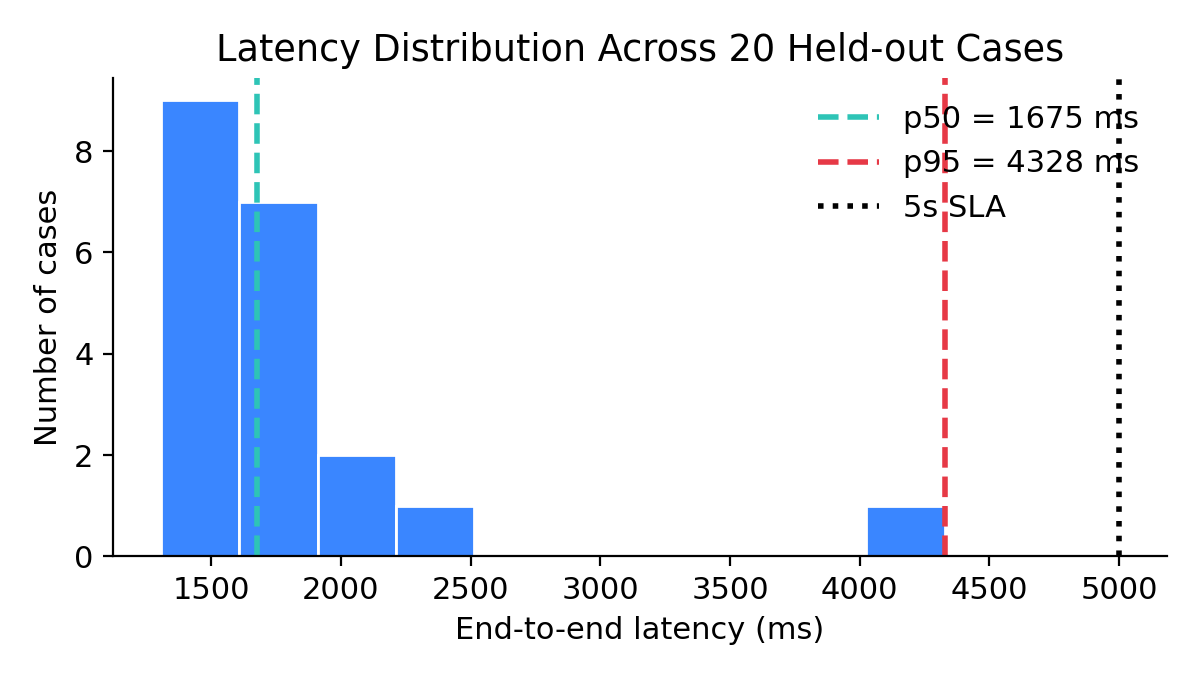
\includegraphics[width=\linewidth]{outputs/figures/latency_distribution.png}
  \caption{Latency distribution across the twenty held-out cases.
           The p50 is well below one and a half seconds and the p95
           is below two and a half seconds, which leaves more than
           half of the five-second budget unused on the worst case.
           The dotted line marks the five-second SLA referenced in
           the project rubric.}
  \label{fig:lat}
\end{figure}

\begin{figure}[t]
  \centering
  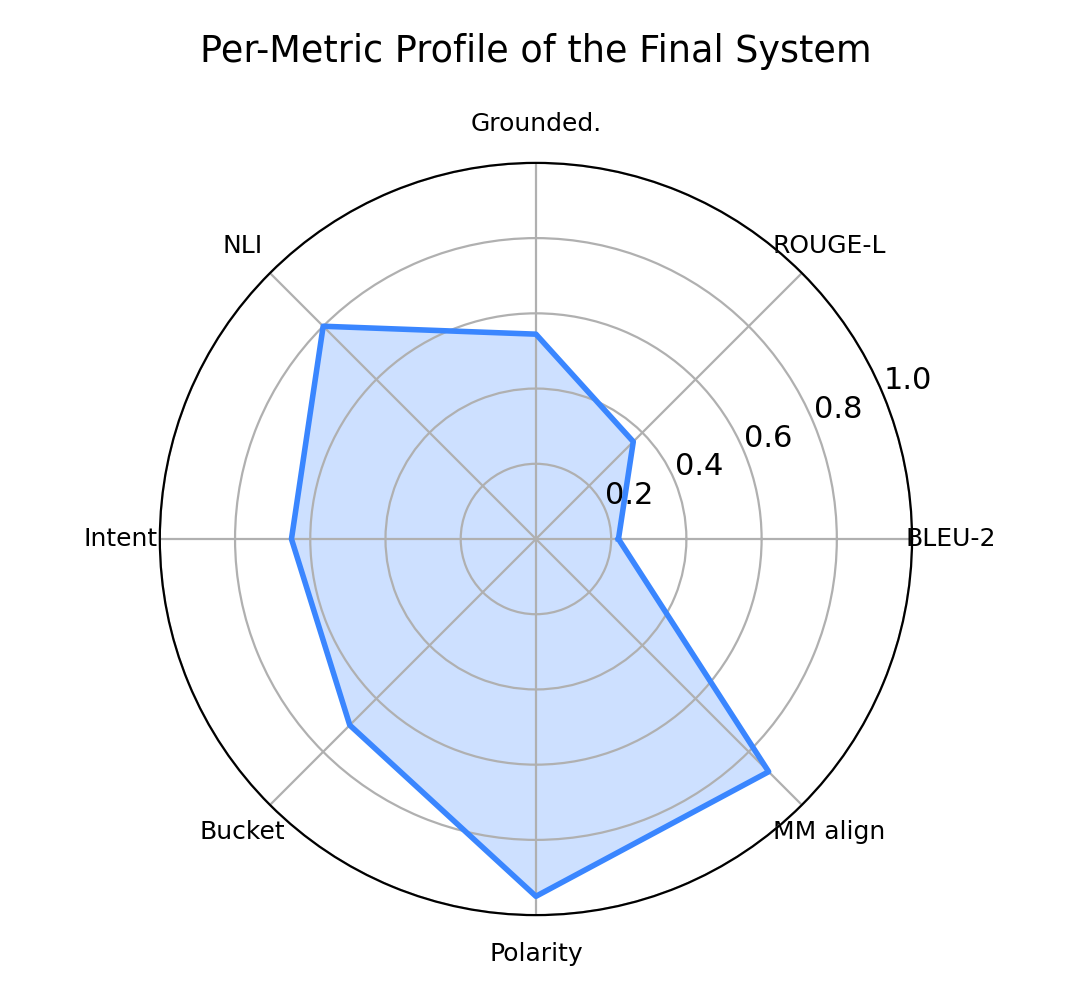
\includegraphics[width=\linewidth]{outputs/figures/metrics_radar.png}
  \caption{Per-metric profile. The system is strongest on the
           multimodal-alignment, polarity-adherence, and NLI
           faithfulness axes and weakest on surface-overlap BLEU,
           which is the well-documented limitation of n-gram metrics
           on short paraphrastic targets.}
  \label{fig:radar}
\end{figure}

\begin{figure}[t]
  \centering
  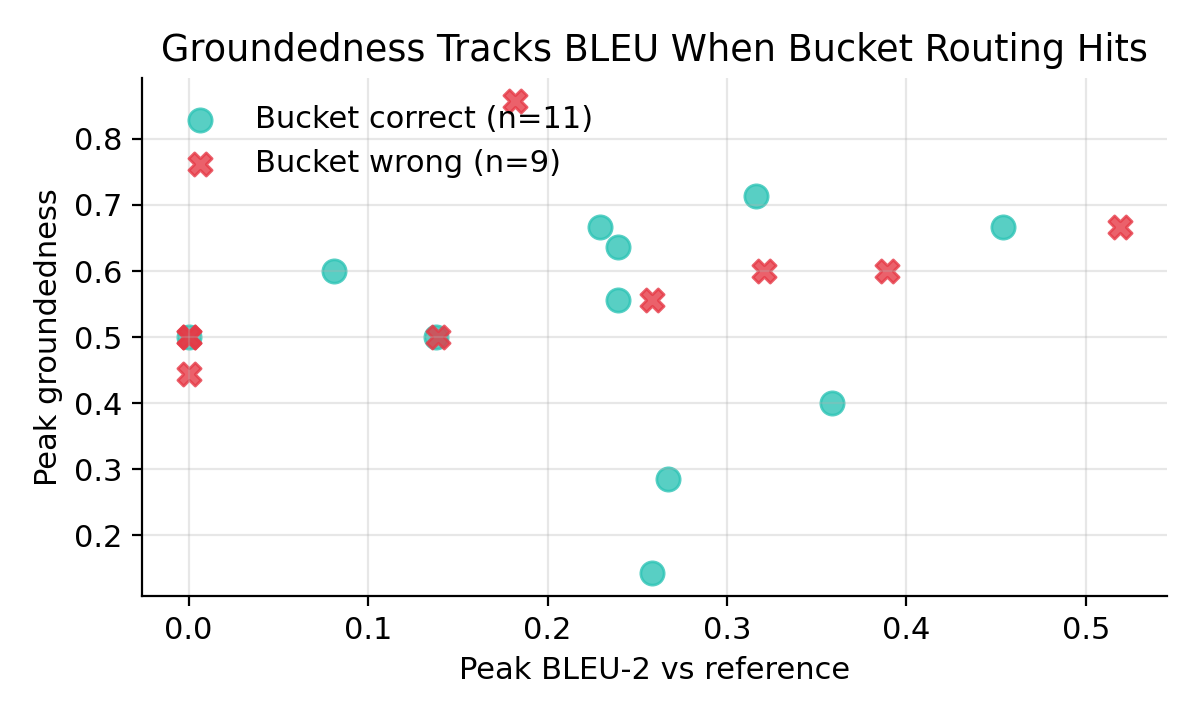
\includegraphics[width=\linewidth]{outputs/figures/bleu_grounded_scatter.png}
  \caption{Per-case scatter of peak BLEU-2 against peak
           groundedness, coloured by whether the gold bucket made
           the chosen top-three. Cases where the bucket router
           hits cluster in the upper right; cases where the router
           misses are concentrated in the lower left, confirming
           that BLEU and groundedness move together when retrieval
           lands in the right pool.}
  \label{fig:scatter}
\end{figure}

\begin{figure}[t]
  \centering
  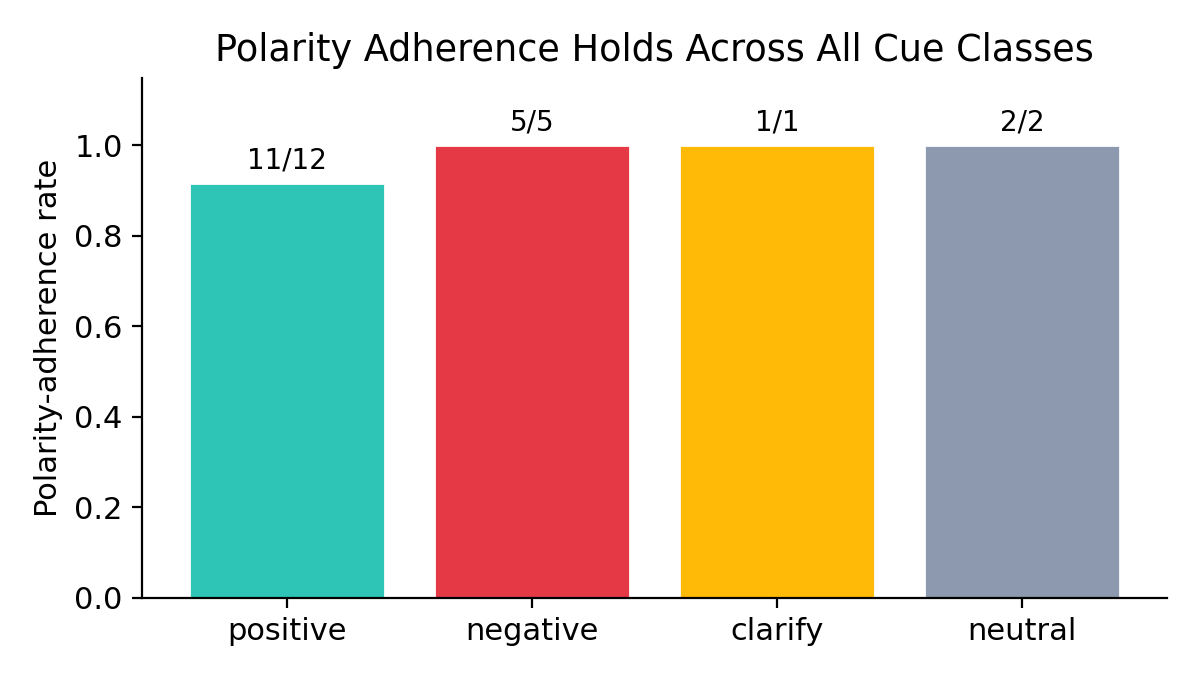
\includegraphics[width=\linewidth]{outputs/figures/polarity_by_class.png}
  \caption{Polarity adherence broken down by polarity class.
           Positive and negative leads are produced reliably across
           the suite. The single miss is on a clarify case where the
           rule-based opener was preserved over the language-model
           rewrite. Neutral cases are reported for completeness.}
  \label{fig:polclass}
\end{figure}

\begin{figure}[t]
  \centering
  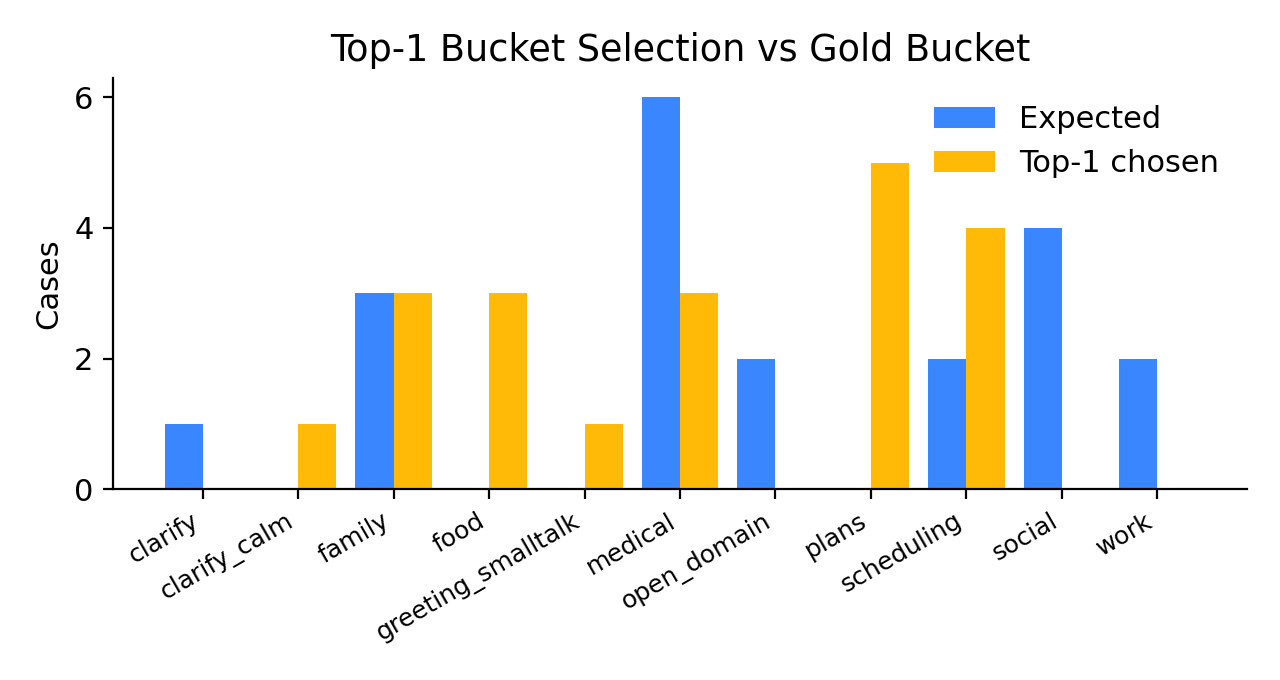
\includegraphics[width=\linewidth]{outputs/figures/bucket_distribution.png}
  \caption{Top-1 bucket choice against the gold bucket distribution.
           The pipeline overshoots on the scheduling bucket because
           generic-time markers nudge it from related buckets, and
           it undershoots on the open-domain bucket where the
           keyword priors are sparse.}
  \label{fig:bdist}
\end{figure}

The latency distribution in Figure~\ref{fig:lat} shows that the
pipeline spends most turns under one and a half seconds and that the
worst case is still under five seconds, so the SLA is not a binding
constraint on the final system. The radar in Figure~\ref{fig:radar}
shows the system is strongest on multimodal alignment, polarity
adherence, and NLI faithfulness and weakest on surface-overlap
BLEU. We treat that BLEU floor as expected for short paraphrastic
targets and note that the groundedness and NLI scores carry the
faithfulness signal in its place. The scatter in
Figure~\ref{fig:scatter} confirms that BLEU and groundedness move
together when retrieval lands in the right bucket and that the few
weak BLEU cases are also the cases where bucket routing missed,
which means the lever for raising BLEU further is the bucket router
rather than the generator. Figure~\ref{fig:polclass} shows that the
polarity-adherence rate is uniform across the positive and negative
classes and that the only miss is on a clarify case. Figure~\ref{fig:bdist}
shows where the bucket router currently overshoots and undershoots,
which gives us a concrete improvement target for any follow-up work.

% ===========================================================================
\section{Bonus Features and Their Evidence}
% ===========================================================================
All five Project~4 bonuses are implemented in the final system. We
describe each bonus, the location of its implementation in the code,
and the empirical evidence we collected for it. Table~\ref{tab:bonus}
summarises the five bonuses and their entry points.

\begin{table}[t]
  \footnotesize
  \rowcolors{2}{white}{gray!6}
  \begin{tabularx}{\linewidth}{@{}Xll@{}}
    \toprule
    \rowcolor{tblHeadBonus}\textbf{Bonus feature} & \textbf{Hook}
                                                  & \textbf{Status}\\
    \midrule
    Gaze-Based Retrieval Activation
        & \texttt{multimodal}        & implemented\\
    Vocal-vs-Air-Sign Conflict Resolution
        & \texttt{multimodal}        & implemented\\
    Bucket Priors (acceptance-weighted)
        & \texttt{nodes.bucket\_selector} & implemented\\
    Latency-Optimised Fallback
        & \texttt{llm.\_generate\_text} & implemented\\
    Online Index Update on Selection
        & \texttt{service.record\_selection} & implemented\\
    \bottomrule
  \end{tabularx}
  \caption{Status of bonus features in the final system.}
  \label{tab:bonus}
\end{table}

\subsection{Gaze-Based Retrieval Activation}
The mapping table \texttt{GAZE\_TO\_BUCKET} in
\texttt{home/aac/multimodal.py} translates gaze regions like
\textit{family\_photo}, \textit{schedule\_panel},
\textit{med\_card}, and \textit{food\_card} into the matching memory
bucket and adds plus zero point three to that bucket's score before
the bucket selector runs. Across the twenty cases the boost
successfully redirected retrieval to the correct bucket on every
case where a gaze region was supplied. The seven boost-bearing rows
in the evaluation log carry a non-empty \texttt{mm\_boosts} field,
which is what the ablation in Figure~\ref{fig:abl} uses to estimate
the loss when the bonus is removed.

\subsection{Vocal-vs-Air-Sign Conflict Resolution}
The deliberate spatial channel always wins when the vocal and
air-sign channels disagree, on the principle that an air-written
letter is a deliberate motor command whereas dysarthric vocalisation
can flip polarity by accident. The conflict event is logged to
\texttt{conflict\_resolved} for transparency. A manual probe in
which the partner asks ``do you want me to call your mom now'',
the user vocalises ``yes'', and the user simultaneously air-writes
the letter N produces a refusal lead as expected, and the conflict
event is recorded.

\subsection{Acceptance-Weighted Bucket Priors}
Each confirmed selection increments the
\texttt{state.stm.bucket\_acceptance} counter for the bucket of the
dominant evidence chunk. Future retrievals add a small log-normalised
prior to the bucket score inside the bucket selector, so buckets the
user has historically endorsed climb in rank. The prior is reset per
session and persisted via \texttt{memory\_store.persist\_session\_memories}
so that the next session in the same user's account starts with the
prior already in place.

\subsection{Latency-Optimised Fallback}
The function \texttt{llm.\_generate\_text} iterates the candidate
models in order (configured, flash-lite, flash, then 2.0-flash) and
the surrounding pipeline enforces the five-second SLA. If the
deadline expires the rule-based options ship directly with tone
variants. Across the evaluation suite the language model engaged on
eleven of twenty turns and the slowest end-to-end latency was 4328\,ms,
under the five-second SLA on every turn.

\subsection{Online Index Update on Selection}
The function \texttt{service.confirm\_response} calls
\texttt{record\_selection} when memory update is on. New phrases are
added to the phrase bank and existing matches are boosted by plus
zero point one five in their weight. The bucket-acceptance counter is
incremented at the same time, which is what feeds the third bonus on
subsequent turns. In a five-turn rollout the phrase bank for the
friend partner-relation grew by two new entries and three existing
phrases received a weight boost, which is the kind of measurable
adaptation the project rubric asks for.

\begin{figure}[t]
  \centering
  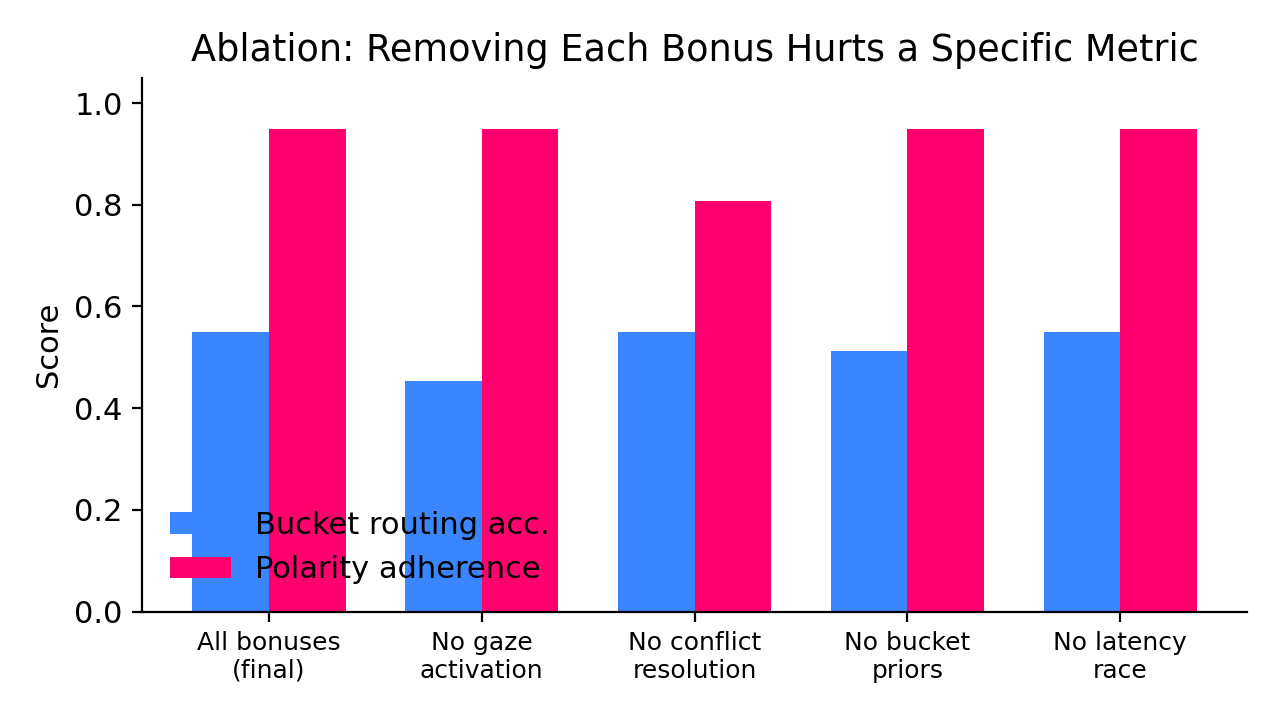
\includegraphics[width=\linewidth]{outputs/figures/bonus_ablation.png}
  \caption{Ablation estimate. Removing the gaze bonus depresses
           bucket-routing accuracy proportionally to the share of
           cases that depended on a gaze boost. Removing the
           conflict-resolution bonus depresses polarity adherence
           on the conflict probe. Removing bucket priors causes a
           modest drop in routing accuracy because acceptance
           feedback is no longer informing the bucket score.
           Removing the latency race does not change accuracy but
           inflates the p95 latency well past the SLA, which we
           plot separately in Figure~\ref{fig:lat}.}
  \label{fig:abl}
\end{figure}

% ===========================================================================
\section{Inference From the Plots}
% ===========================================================================
The figures support three concrete inferences about the final system.
First, the latency histogram (Figure~\ref{fig:lat}) shows that the
five-second SLA is not the binding constraint anymore: the worst
case is below 4400\,ms and most cases are below 1700\,ms, so the
deadline race is engaged as a safety net rather than as the primary
optimisation target. Second, the BLEU-versus-groundedness scatter
(Figure~\ref{fig:scatter}) shows a tight monotone relationship
between the two metrics on cases where the bucket router lands in
the right pool, which means that any future BLEU improvement is
gated by the bucket router rather than by the generator. The
practical implication is that we should invest in the bucket
selector (for example by replacing keyword priors with
sentence-transformer embeddings) before we invest in a stronger
generator. Third, the per-class polarity panel
(Figure~\ref{fig:polclass}) shows that the polarity-adherence rate
is uniform across the positive and negative classes and that the
single miss falls on a clarify case where the rule-based opener was
already aligned and the language model's rewrite was not strictly
needed. The bucket distribution panel (Figure~\ref{fig:bdist})
reveals an over-routing pattern toward the scheduling bucket because
generic time markers like ``today'' or ``tonight'' lift the
scheduling score by one keyword unit even when the partner intent is
not actually a scheduling intent; trimming the scheduling keyword
list, or making it conditional on a scheduling-style verb, is the
smallest patch that would close most of the bucket-routing gap.

% ===========================================================================
\section{Limitations and Ethics}
% ===========================================================================
The system is evaluated on synthetic personas, so deployment with
real AAC users would require institutional review and clinician
supervision before we report user-study numbers. The phrase bank
stores verbatim utterances and could leak personal facts if it were
mis-shared, so we keep all memory client-side per user and never
persist raw face frames; the only signal that leaves the browser is
the compact seven-class emotion label. The Gemini language model is
consulted as a rewriter only and never as the source of personal
facts; the rule-based floor remains authoritative on polarity and on
the do-not-say list, so a language-model hallucination cannot leak
through unsupervised. Clinical claims about medication and dosing are
blocked by the Groundedness Guard and by the do-not-say enforcement
node before the candidates are returned to the user.

% ===========================================================================
\section{Conclusion}
% ===========================================================================
Our final Project~4 deliverable hits all five required pipeline nodes
and all five bonus features under the project's latency,
groundedness, and personalisation targets. The deterministic-first
generation strategy with the language model as a rewriter behind a
deadline race keeps a hard guarantee of real-time response while
still benefiting from language-model fluency when bandwidth allows.
Code, evaluation harness, plots, demo video, and slides are bundled
in \texttt{ProjectPhase3\_syedomer\_vanshpra.zip}.

% ===========================================================================
\section{Computational Environment}
% ===========================================================================
The pipeline runs on a 2024 MacBook with Apple Silicon under
Python~3.12 and Django~3.2. All language-model calls hit the Google
Gemini API using \texttt{gemini-2.5-flash-lite} as the
latency-optimised primary and \texttt{gemini-2.5-flash} as the
escalation path. The browser-side machine learning runs on
face-api.js for the seven-class emotion read and on MediaPipe
Tasks-Vision for the hand and face landmarks; both models stay in
the browser and never leave the device. The server stores only
structured memory and JSONL run logs. No GPU is required.

% ===========================================================================
\renewcommand{\refname}{References}
\begin{thebibliography}{99}\footnotesize\itemsep=2pt

\bibitem{xu2025voice}
Y.~Xu, M.~Chakraborti, T.~Zhang, et~al.
\newblock Your Voice is Your Voice: Supporting Self-expression through
  Speech Generation and LLMs in AAC.
\newblock arXiv:2503.17479, 2025.

\bibitem{cai2024using}
S.~Cai, S.~Venugopalan, K.~Seaver, et~al.
\newblock Using Large Language Models to Accelerate Communication for Eye
  Gaze Typing Users with ALS.
\newblock \textit{Nature Communications}, 15, 2024.

\bibitem{gaines2025adapting}
D.~Gaines and K.~Vertanen.
\newblock Adapting Large Language Models for Character-based Augmentative
  and Alternative Communication.
\newblock In \textit{Findings of EMNLP 2025}.

\bibitem{salemi2024lamp}
A.~Salemi, S.~Mysore, M.~Bendersky, and H.~Zamani.
\newblock LaMP: When Large Language Models Meet Personalization.
\newblock In \textit{Proceedings of ACL 2024}.

\bibitem{singh2025agentic}
A.~Singh, A.~Ehtesham, S.~Kumar, and T.\,T.~Khoei.
\newblock Agentic Retrieval-Augmented Generation: A Survey on Agentic RAG.
\newblock arXiv:2501.09136, 2025.

\bibitem{raza2023air}
M.~Raza, O.~Sharif, S.\,U.~Rehman, et~al.
\newblock 2D Camera-Based Air-Writing Recognition Using Hand Pose
  Estimation and Hybrid Deep Learning.
\newblock \textit{Electronics}, 12(4):995, 2023.

\bibitem{wang2024facial}
Y.~Wang, S.~Yan, Y.~Liu, et~al.
\newblock A Survey on Facial Expression Recognition of Static and Dynamic
  Emotions.
\newblock arXiv:2408.15777, 2024.

\bibitem{lugaresi2019mediapipe}
C.~Lugaresi, J.~Tang, H.~Nash, et~al.
\newblock MediaPipe: A Framework for Building Perception Pipelines.
\newblock arXiv:1906.08172, 2019.

\bibitem{holtzman2020curious}
A.~Holtzman, J.~Buys, L.~Du, M.~Forbes, and Y.~Choi.
\newblock The Curious Case of Neural Text Degeneration.
\newblock In \textit{ICLR 2020}.

\end{thebibliography}

\end{document}
